\documentclass[12pt]{article}
\usepackage{fontspec}
\usepackage{graphicx}
\usepackage{geometry}
\usepackage{lipsum}
\usepackage[czech]{babel}
\usepackage{titling}
\usepackage{xevlna}
\usepackage{textgreek}
\usepackage{amsmath}
\usepackage[section]{placeins}
\renewcommand\maketitlehooka{\null\mbox{}\vfill}
\renewcommand\maketitlehookd{\vfill\null}

\usepackage{fontspec}
\setmainfont[Mapping=tex-text]{Times New Roman}
\newfontface\TVSp{DejaVu Serif}
\def\textvisiblespace{{\TVSp\char"2423}}


\setlength{\parindent}{0pt} 
 
\title{MI--SPI Druhá úloha}
\author{Tomáš Pšenička, Jan Groschaft}
\date{\today}
 
 
 % Definition of \maketitle
\makeatletter         
\def\@maketitle{
%\raggedright
\begin{center}
{\Huge \bfseries \sffamily \@title }\\[4ex] 
{\Large  \@author}\\[4ex] 
\@date\\[8ex]

\includegraphics[width = 60mm]{symbol_cvut_plna_samostatna_verze_cb.pdf}
\end{center}}
\makeatother

% \makeatletter
% \renewcommand\thesection{}
% \renewcommand\thesubsection{\@arabic\c@section.\@arabic\c@subsection}
% \makeatother


\begin{document}
 
\begin{titlingpage}
	\maketitle
\end{titlingpage}
 	
	\newpage
 
	\tableofcontents

	\newpage

 	\section{Zadání}
 	
 	\begin{itemize}
 		\item Z obou datových souborů načtěte texty k analýze. Pro každý text zvlášť odhadněte základní charakteristiky délek slov, tj. střední hodnotu a rozptyl. Graficky znázorněte rozdělení délek slov.
  		\item Pro každý text zvlášť odhadněte pravděpodobnosti písmen (symbolů mimo mezery), které se v textech vyskytují. Výsledné pravděpodobnosti graficky znázorněte.
 		\item Na hladině významnosti 5\% otestujte hypotézu, že rozdělení délek slov nezávisí na tom, o který jde text. Určete také p-hodnotu testu. 		
 		\item Na hladině významnosti 5\% otestujte hypotézu, že se střední délky slov v obou textech rovnají. Určete také p-hodnotu testu.
		\item Na hladině významnosti 5\% otestujte hypotézu, že rozdělení písmen nezávisí na tom, o který jde text. Určete také p-hodnotu testu.
 	\end{itemize}
   		
   		
	\section{Řešení}\label{r}
		\subsection{Charakteristika délek slov}\label{pz}
            Pro odhad charakteristik délek slov jsme použili výběrový průměr a výběrový rozptyl: 
               $$\bar{X}_n = \frac{1}{n} \sum_{i}{X_i}$$   					
               $$s_n^2 = \frac{1}{n-1} \sum_{i}{(X_i - \bar{X}_n)^2}$$.
            Výsledky sledujeme v tabulce~\ref{stat-table} a na obrázcích~\ref{009_graph} a~\ref{011_graph}. 

	\begin{table}[!ht]
\centering
\begin{tabular}{ | c | l | l | } \hline
Text	& $\bar{X}_n$ & $s_n^2$ \\ \hline
009.txt & 4.2623 & 4.9860 \\  \hline
011.txt & 3.8603 & 4.5360 \\ \hline
\end{tabular}
\caption{Charakteristika délek slov}
\label{stat-table}
\end{table}

\begin{figure}[!ht]
  \centering
       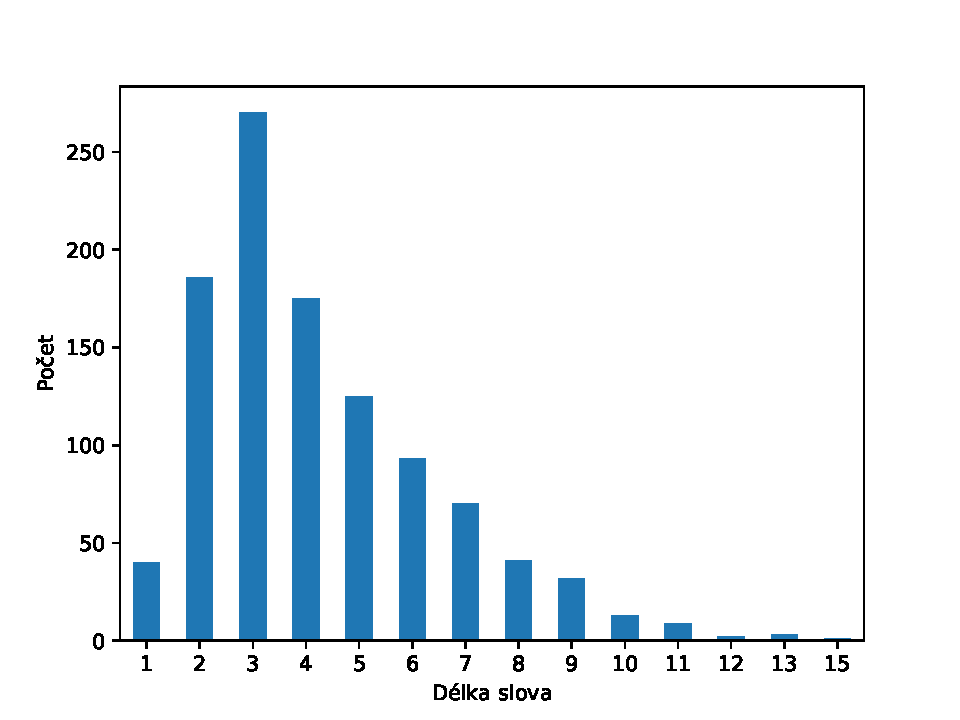
\includegraphics[width=1.0\textwidth]{hw2_plot1_009.pdf}
        \caption{Rozdělení délek slov v souboru 009.txt}
        \label{009_graph}
  \end{figure}
\begin{figure}[!ht]
  \centering
       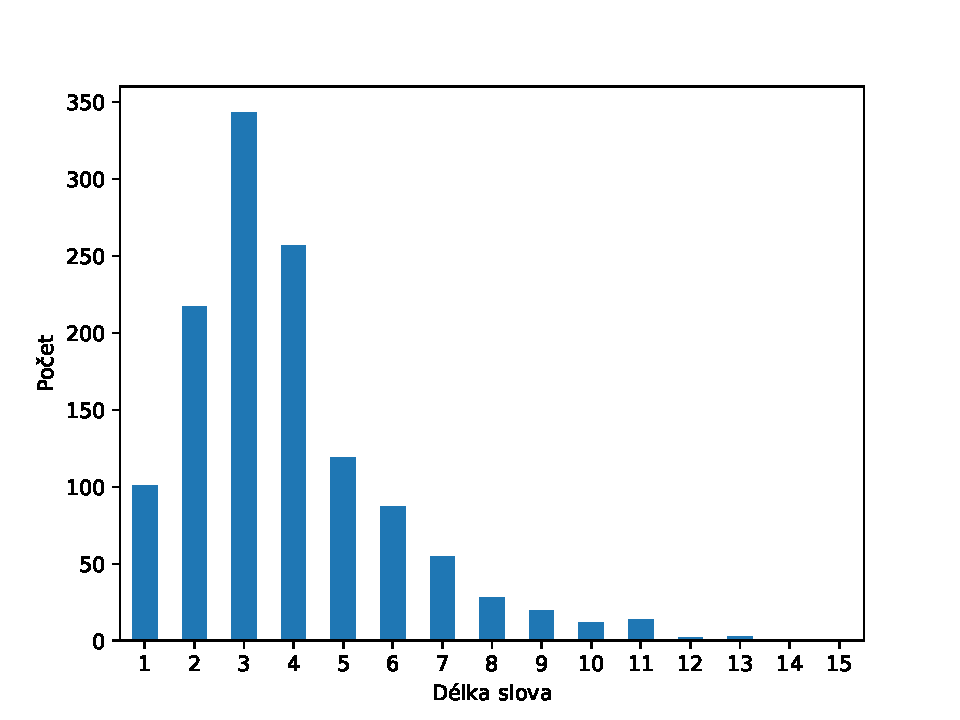
\includegraphics[width=1.0\textwidth]{hw2_plot1_011.pdf}
        \caption{Rozdělení délek slov v souboru 011.txt}
        \label{011_graph}
  \end{figure}

				\subsection{Pravděpodobnosti znaků}\label{pz}
			 Pravděpodobnost jednotlivých znaků byla vypočítána jako poměr počtu výskytů jednotlivých znaků k celkovému počtu všech znaků a je znázorněna v grafech \ref{009_graph2} a \ref{011_graph2} pomocí nástroje matplotlib.
						
\begin{figure}[!htb]
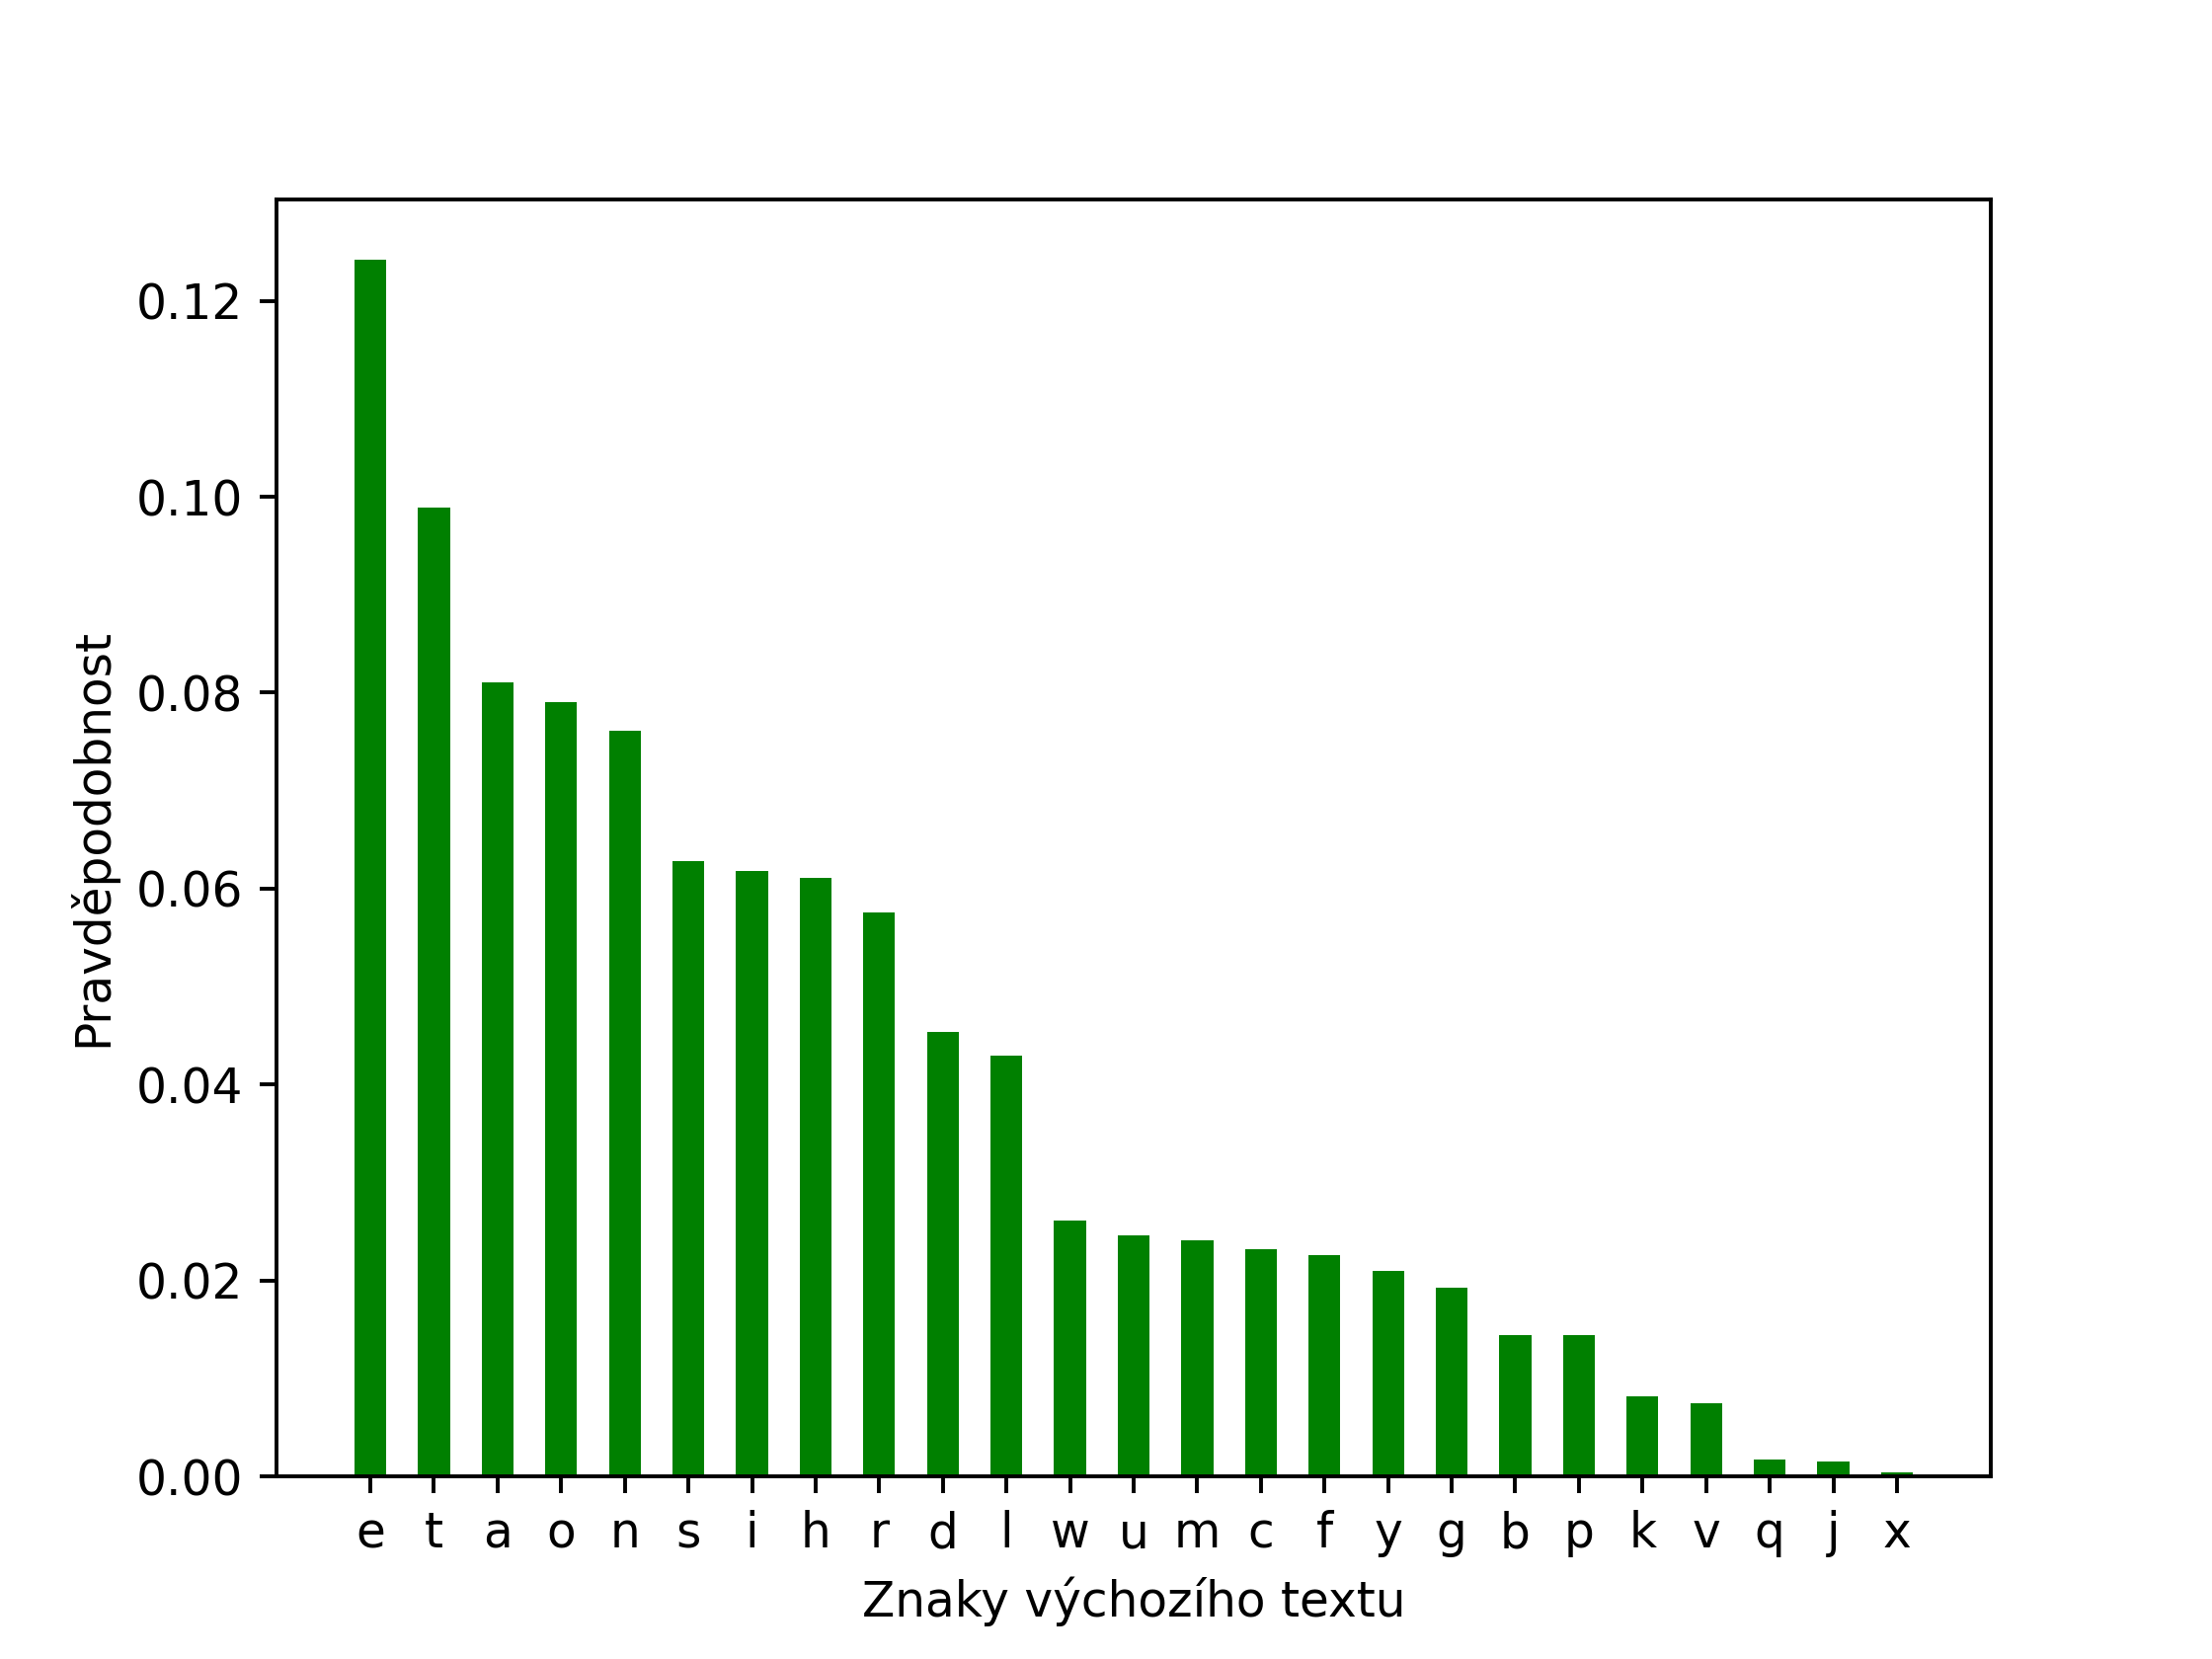
\includegraphics[scale=0.8]{009_char_prob.png}\centering\caption{Grafické znázornění pravděpodobností znaků textu 009.txt}\label{009_graph2}
\end{figure}

\begin{figure}[!htb]
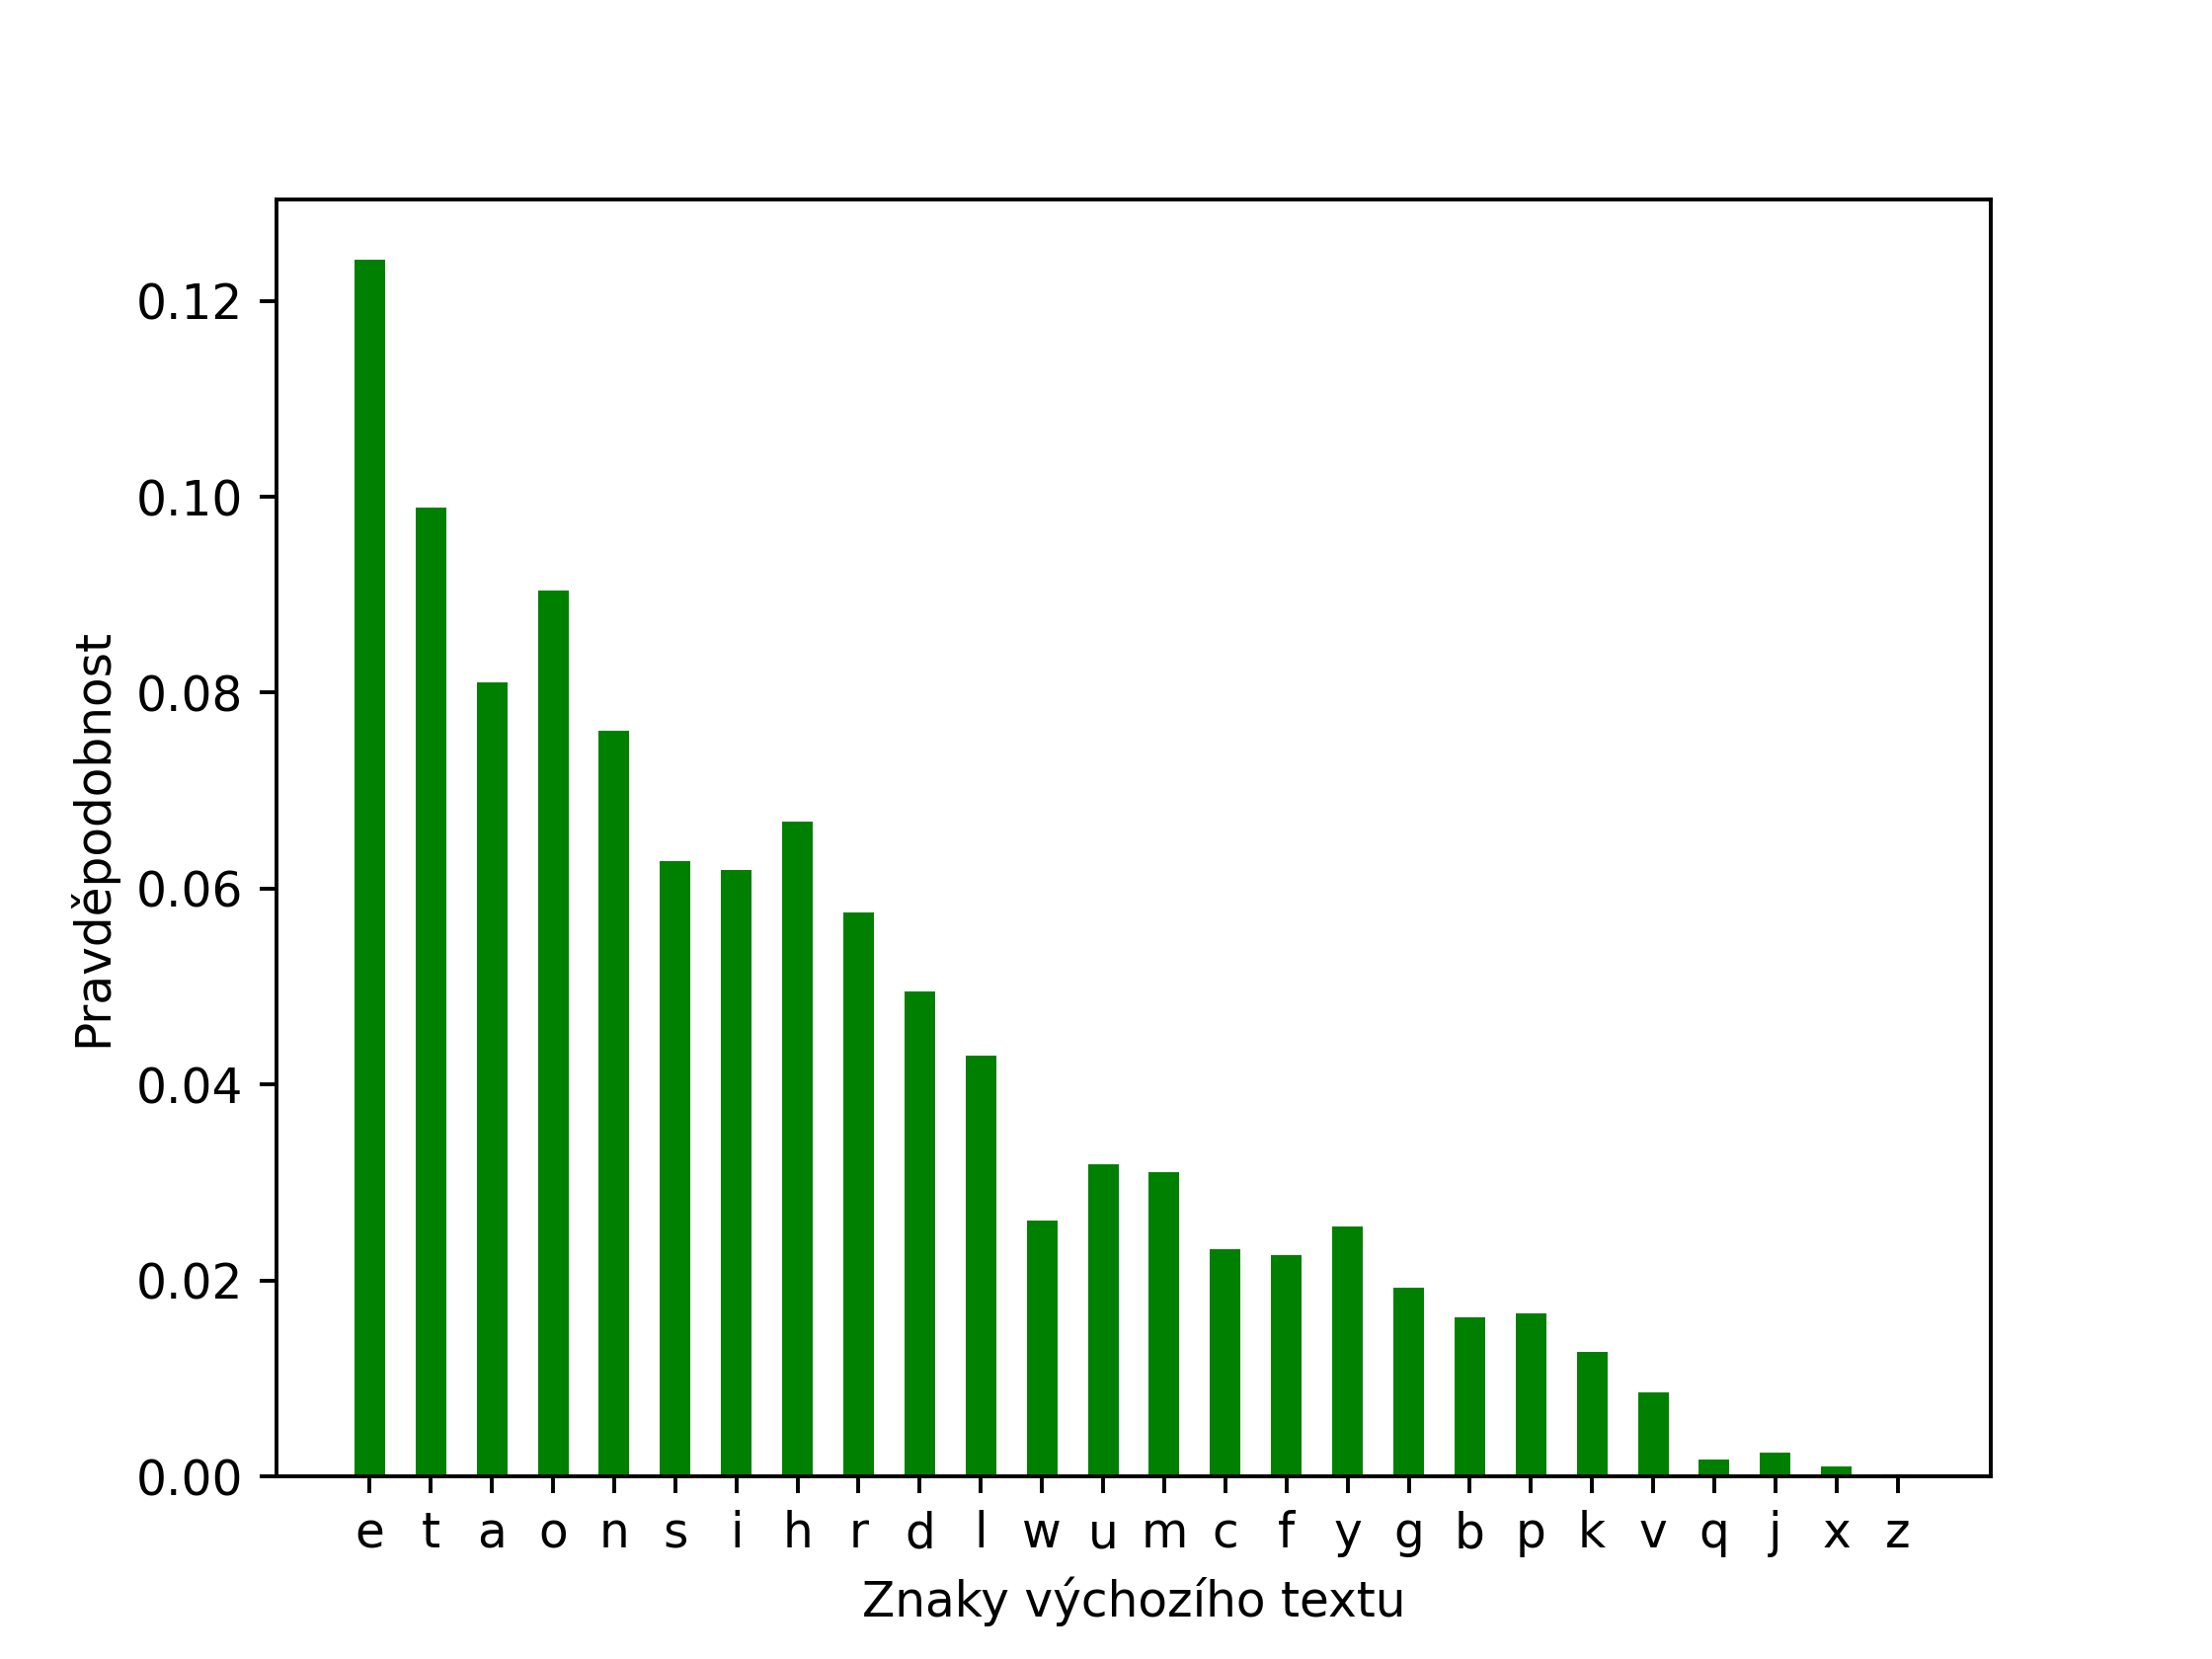
\includegraphics[scale=0.8]{011_char_prob.png}\centering\caption{Grafické znázornění pravděpodobností znaků textu 011.txt}\label{011_graph2}
\end{figure}

    \subsection{Na hladině významnosti 5\% otestujte hypotézu, že rozdělení délek slov nezávisí na tom, o který jde text. Určete také p-hodnotu testu.}	
		
    Provedli jsme test nezávislosti v kontingenční tabulce, viz tabulku~\ref{Cont_table1}. Testujeme hypotézu $H_0$, že rozdělení délek slov nezávisí na volbě zdrojového textu oproti alternativě $H_A$, že na volbě zdrojového textu závisí. \\
Testová statistika $\chi^2$ má tvar
$$\chi^2 = n\sum_{i =1}^r\sum_{j=1}^c \frac{N_{i,j}^2}{N_{i, \bullet}N_{\bullet, j}}$$
a po dosazení $r=2, c=15$ máme $\chi^2 = 45.6235$ a p-hodnotu $3.2990e-05$

Kritická hodnota je $\chi^2_{\alpha, (r-1)(c-1)} = \chi^2_{0.05, 14} = 23.68$. Protože je naše testová statistika větší než kritická hodnota, zamítáme nulovou hypotézu ve prospěch alternativy.

\subsection{Na hladině významnosti 5\% otestujte hypotézu, že se střední délky slov v obou textech rovnají. Určete také p-hodnotu testu.}
Cheme testovat hypotézu $H_0: \mu_1 = \mu_2$ proti $H_A: \mu_1 \neq \mu_2$. Použijeme dvouvýběrový t-test za předpokladu různých rozptylů, tedy $\sigma_1 \neq \sigma_2$.\\
Použijeme tedy konkrétně testovou statistiku 
$$T = \frac{\bar{X}_n - \bar{Y}_n}{s_d},$$
kde
$$s_d = \sqrt{\frac{s_X^2}{n}+\frac{s_Y^2}{m}}$$

Po dosazení vychází $T = -4.409004682120487$ a p-hodnota je $1.0882e-05$

    \begin{table}[!ht]
    \centering
    \begin{tabular}{|l|rrrrrrrrrrrrrrr|} \hline
Soubor &  1  &   2  &   3  &   4  &   5  &  6  &  7  &  8  &  9  &  10 &  11 &  12 &  13 & 14 & 15 \\ \hline
009.txt &  40 &  186 &  270 &  175 &  125 &  93 &  70 &  41 &  32 &  13 &   9 &   2 &   3 & 0 &  1 \\ \hline
011.txt &  101 &  217 &  343 &  257 &  119 &  87 &  55 &  28 &  20 &  12 &  14 &   2 &   3 &   1 &   1 \\ \hline

\end{tabular}
\caption{Kontingenční tabulka četností délek slov}
\label{Cont_table1}
\end{table}
	
   	\section{Závěr}\label{z}
   		

\end{document}
